Hallar el volumen del toroide que se genera al girar la curva $(x-3)^2+y^2=4$ alrededor del eje $x$.

\nopagebreak
\begin{align*}
\text{Círculo centro } (3,0), \text{radio } 2. \text{ Rotación alrededor del eje } y. \\
\text{Es un Toroide. Usamos Teorema de Pappus.} \\
V &= 2\pi R \cdot A \\
R &= 3 \text{ (distancia del centro al eje } y). \\
A &= \pi r^2 = \pi (2)^2 = 4\pi. \\
V &= 2\pi (3) (4\pi) = 24\pi^2
\end{align*}

\[
\boxed{\displaystyle 24\pi^2}
\]

\begin{center}
    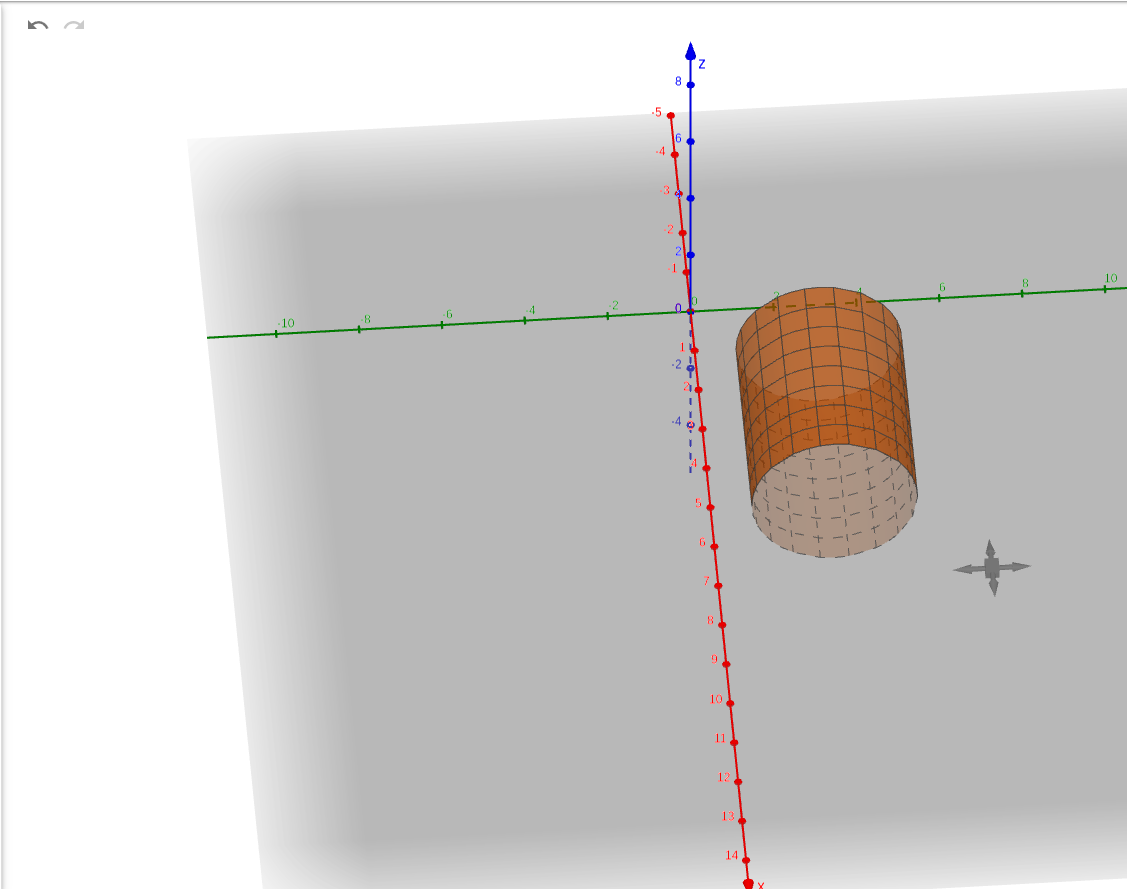
\includegraphics[width=0.5\textwidth]{Graficas/ejer35.png}
\end{center}
